\chapter[Projekt und Organisation]{Projekt und Organisation\footnote{Jens Helge Micke}}
\thispagestyle{fancy}
\label{ProjektOrganisation}
Inhalt dieses Kapitels ist die Vorstellung des Projektes und die Organisation der Gruppe 5.
\section{Das Projekt}
\label{DasProjekt}
Die Entwicklung eines Server-Client Systems zur Darstellung PDF-basierter Präsentationen kristallisierte sich nach der Abwägung anderer Projektmöglichkeiten\footnote{Besprochene Alternativen: Ein kooperatives Jump 'n Run Spiel, Medienserver} heraus.
Auch, dass der ausgehändigte \glqq Raspberry Pi 3 \grqq als Server und, in Verbindung mit einer HDMI-fähigen Anzeige, als Primäranzeige dienen soll ergab sich als natürliche Rahmenbedingung.
\subsection{Anwendungsfälle}
\label{Anwendungsfälle}
Bevor es an die Verteilung von Aufgaben innerhalb des Projektes ging wurden die entsprechenden Anwendungsfälle erarbeitet.
Während der Realisierung wurden diese an die derzeitige Situation angepasst und nötigenfalls Erweitert.\\


\begin{tabularx}{\textwidth}[!htb]{|l|X|}
	\hline
	1.0 & Präsenter \\
	 & Mehrere Personen wollen eine Präsentation halten \\
	\hline
	\hline
	1.1 & PräsenterEinwahl\\
	& Präsenter wählt sich in das System ein\\
	\hline
	\hline
	1.2 & PräsentationHochladen\\
	& Präsenter lädt Präsentation hoch\\
	VORRAUSSETZUNG & 1.1 PräsenterEinwahl\\
	\hline
	\hline
	1.3 & PräsentationAnzeigen\\
	& Die Präsentation wird angezeigt\\
	VORRAUSSETZUNG & 1.2 PräsentationHochladen\\
	\hline
	\hline
	1.4 & Navigation\\
	& Präsenter navigiert Präsentation\\
	BEFEHLE & vor, zurück\\
	VORRAUSSETZUNG & 1.3 PräsentationAnzeigen\\
	BESCHRÄNKUNG & Anfang/Ende der Präsentation\\
	BESCHRÄNKT & 2.2 PräsentationAnzeigen\\
	\hline
	\hline
	1.4.1 & NavigationSchaltflächen\\
	& Benutzeroberfläche stellt NavigationSchaltflächen bereit\\
	BEFEHLE & wie 1.3\\
	\hline
	\hline
	1.4.2 & NavigationBeschleunigungssensor\\
	& Navigation durch Kippbewegungen\\
	BEFEHLE & zurück, vor\\
	BESCHRÄNKUNG & Orientierung des Geräts\\
	\hline
	\hline
	1.4.3 & NavigationMikrofon\\
	& Navigation durch Klopfzeichen\\
	BEFEHLE & 1x Klopfen = vor\\
	& 2x Klopfen = zurück\\
	\hline
	\hline
	1.4.5 & NavigationKamera\\
	& Kamera erkennt Gesten zur Navigation\\
	BEFEHLE & Bewegung nach links = zurück\\
	& Bewegung nach rechts = vor\\
	\hline
	\hline
	1.5 & Menue\\
	& Navigationsmöglichkeiten 1.4.x x>1 an/abschalten\\
	& Die Präsentation kann beendet werden.\\
	& Eine neue Präsentation kann gestartet werden.\\
	\hline
\end{tabularx}

\begin{tabularx}{\textwidth}[!htb]{|l|X|}
	\hline
	2.0 & Publikum\\
	& Mehrere Personen wollen eine Präsentation verfolgen\\
	\hline
	\hline
	2.1 & PublikumEinwahl\\
	& Publikumsperson wählt sich in das System ein\\
	\hline
	\hline
	2.2 & PräsentationAnzeigen\\
	& Die Präsentation wird angezeigt\\
	VORRAUSSETZUNG & 1.3 PräsentationHochladen\\
	& 2.1 PublikumEinwahl\\
	\hline
	\hline
	2.3 & PräsentationSpeichern\\
	& Die Präsentation wird gespeichert\\
	VORRAUSSETZUNG & 1.3 PräsentationHochladen\\
	& 2.1 PublikumEinwahl\\
	\hline
	\hline
	2.4 & Verlassen\\
	& Die Publikumsperson verlässt die Präsentation\\
	VORRAUSSETZUNG & 2.1 PublikumEinwahl\\
	\hline
	\hline
	2.5 & Menue\\
	& Ein Menue erlaubt die Anwendungsfälle 2.1 - 2.4\\
	\hline
\end{tabularx}

\begin{tabularx}{\textwidth}[!htb]{|l|X|}
	\hline
	3.0 & DienstAnforderungen\\
	\hline
	\hline
	3.1 & Benutzer/Rechteverwaltung\\
	& Mehrere Präsenter\\
	& Mehrere passwörgeschützte Publikumspersonen\\
	\hline
	\hline
	3.2 & Datenverwaltung\\
	& Sortierung und Verwaltung von Präsentationen\\
	\hline
	\hline
	3.3 & Klientenschnittstelle\\
	& Muss derzeitige Seite der Präsentation verteilen.\\
	\hline
	\hline
	3.4 & Klientenverteilung\\
	& Muss aktuellste Version des Klienten verteilen\\
	\hline
\end{tabularx}

\begin{figure}[!htb]
	\centering
	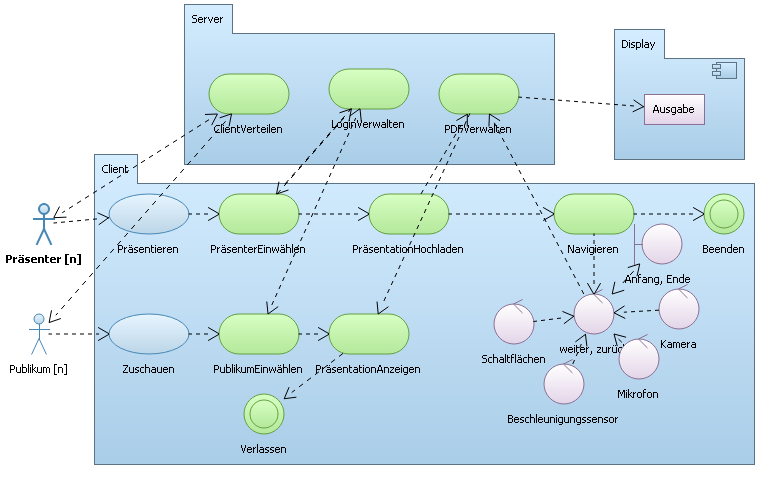
\includegraphics[angle=0,width=14cm]{ProjektOrganisation/Bilder/Anwendungsfaelle.png}
	\caption{Anwendungsfälle}
	\label{BildAnwendungsfaelle}
\end{figure}

\section{Die Organisation}
Aus den Anwendungsfällen in Kapitel \ref{Anwendungsfälle} Seite \pageref{Anwendungsfälle} ff. bzw. Bild \ref{BildAnwendungsfaelle} Seite \pageref{BildAnwendungsfaelle} ließen sich erste Hauptverantwortlichkeiten der Gruppenmitglieder ableiten und verteilen.\\

\begin{tabularx}{\textwidth}[!htb]{|l|X|}
	\hline
	Server & Entwicklung des Servers\\
	\hline
	Klient & Benutzeroberfläche und Serverandbindung \\
	\hline
	Navigation & Navigationsmöglichkeiten\\
	& Berührungsschaltflächen, Kamera, Beschleunigungssensor, Mikrofon\\
	\hline
	Raspberry Pi & Integration auf der Hardware\\
	& Klientenverteilung\\
	\hline
	Dokumentation & Projektdokumentation\\
	\hline
	PDF-Renderer & Bereitstellen des PDF-Renderers\\
	\hline
\end{tabularx}
\\
\begin{tabularx}{\textwidth}[!htb]{|l|X|}
	\hline
	René Beckmann & Server\\
	& Klient Serveranbindung\\
	\hline
	Sascha Brexeler & Klient Benutzeroberfläche\\
	& Navigation Berührungsschaltflächen\\
	\hline
	Diana Castano & Navigation Mikrofon\\
	\hline
	Tim Hebbeler & PDF-Renderer\\
	& Navigation Kamera\\
	\hline
	Jens Helge Micke & Raspberry Pi\\
	& Navigation Beschleunigungssensor\\
	& Dokumentation\\
	\hline
\end{tabularx}
\\
GitHub.com\footnote{https://github.com/BeckmaR/EmbeddedMultimediaSS2016} wurde als Versionsverwaltungsplatform genutzt.\\
Absprachen geschahen über regelmäßige Treffen und Gruppenchat.\\
Die zu bearbeitenden Projektteile wurden in kleinen Modulen entwickelt, getestet und nacheinander zusammengefügt.\\
Zu diesem Zweck traf sich die Gruppe zusätzlich zur Heimarbeit zu mehreren Test- und Programmierwochenenden bei denen die Gruppenmitglieder sich gegenseitig halfen und die bearbeiteten Problemlösungen testeten.\\